\begin{center}
    \textbf{Geração 60}
\end{center}

\begin{figure}[h]
    \centering
    \label{fig:geracao01}
    
    \begin{tabular}{rl}
        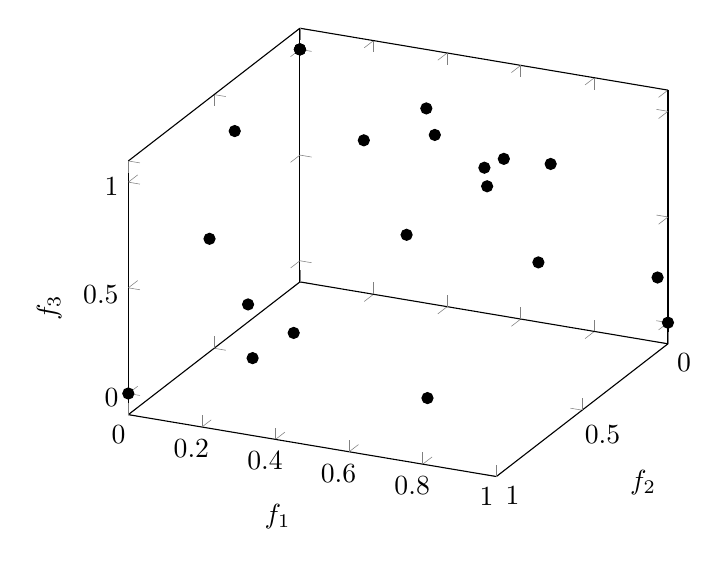
\begin{tikzpicture}[scale=1.0]
        	\begin{axis}[xlabel=$f_2$, ylabel=$f_1$, zlabel=$f_3$, view/h=115]
    			\addplot3[only marks] coordinates {
            		(1.000000, 0.000000, 0.000000) (0.000000, 1.000000, 0.000000) (0.000000, 0.000000, 1.000000) (0.000000, 0.000000, 1.000000) (0.000000, 0.000000, 1.000259) (0.551796, 0.547129, 0.629595) (0.358015, 0.814919, 0.455789) (0.727672, 0.685877, 0.008185) (0.059179, 0.708892, 0.702830) (0.209197, 0.464046, 0.862650) (0.773531, 0.115014, 0.623390) (0.280492, 0.639441, 0.715849) (0.155741, 0.626675, 0.763564) (0.867863, 0.387725, 0.317207) (0.118136, 0.398530, 0.911773) (0.227630, 0.607342, 0.761132) (0.869579, 0.264548, 0.416977) (0.439530, 0.027811, 0.897933) (0.339590, 0.331923, 0.880375) (0.928694, 0.304477, 0.211811) (0.010864, 0.976843, 0.213681) 

        		};
        	\end{axis}
	    \end{tikzpicture}
	    &
	    \begin{tikzpicture}[scale=1.0]
        	\begin{axis}[xlabel=$f_2$, ylabel=$f_1$, zlabel=$f_3$, view={45}{0}]
    			\addplot3[only marks] coordinates {
            		(1.010984,0.000000,0.000000)(0.000000,1.037529,0.000000)(0.000000,0.000000,1.000750)(0.000000,0.000000,1.001416)(0.834344,0.231269,0.523135)(0.708041,0.708917,0.020729)(0.142052,0.333271,0.963492)(0.449248,0.107216,0.891389)(0.514365,0.515286,0.693671)(0.374199,0.827333,0.451951)(0.575647,0.035612,0.818931)(0.431415,0.367960,0.859543)(0.618550,0.586467,0.601420)(0.138000,0.424495,0.920477)(0.591690,0.441873,0.722264)(0.808491,0.024278,0.605166)(0.995947,0.000000,0.178634)(0.983327,0.000000,0.192691)(0.740323,0.551309,0.396134)(0.745135,0.678340,0.241240)(0.247808,0.676069,0.704876) 

        		};
        	\end{axis}
	    \end{tikzpicture}
	\end{tabular}
    
\end{figure}

